\chapter{The Streaming Runtime Library for Cell}\label{ch:lib}

The Cell architecture provides an excellent target for streaming language compilers for a number of reasons:
\begin{itemize}
\item Individual SPEs are optimized for computation.
\item The limited local store available on SPEs is not a severe limitation for actors in a stream program, which are independent, have extremely local data-access patterns, and generally have small code sizes. In an SDF model such as the basic StreamIt model, known static rates further simplify scheduling.
\item The high-bandwidth, low-latency on-chip communication network enables a large number of scheduling options which would not be feasible for other targets, such as computing clusters.
\end{itemize}

The natural division of work on the Cell architecture maps computation to SPEs, which perform DMA operations to copy input and output data to/from local store. In this model, the PPE functions mainly as a control processor, possibly also performing small amounts of computation that are too small to dispatch to an SPE.

Using this model, a streaming language compiler (or programmer) must address four major issues:
\begin{enumerate}
\item Generating highly-SIMDized code in the limited SPE instruction set. SIMD is required to make full use of an SPE's execution units. In addition, code that operates only on vectors avoids rotate instructions needed to load scalar values from local store, in effect producing a greater performance improvement than would be expected.
\item Generating code that performs DMA operations. This code also needs to double-buffer input and output to make full use of Cell's asynchronous communication model.
\item Organizing all needed code and sufficient buffering to fit into limited SPE local store. This is particularly a problem for larger applications, for which the total code size for all filters leaves little room for buffering, or may exceed the size of local store entirely.
\item Performing high-level optimizations and scheduling. At a high level, compilers would typically be interested in balancing workload among available SPEs, avoiding excess communication, transforming code to improve efficiency, and other such topics.
\end{enumerate}

The purpose of the streaming runtime library for Cell is to abstract \textsf{(2)} and provide facilities that simplify \textsf{(3)} and \textsf{(4)}. The library frees a compiler or programmer from needing to deal with the details of Cell's communication model, allowing it to focus on exploring high-level optimization and scheduling choices. The two main functions of the library are:
\begin{itemize}
\item Providing high-level facilities in place of explicit DMA operations between SPE local stores and memory.
\item Providing the \emph{user}\footnote{\emph{User} refers to all non-library code running on the PPE; typically, most of this performs scheduling. Code for filter work functions and auxiliary functions will always be referred to separately.} with a generic framework for controlling and dispatching computation to SPEs that simplifies scheduling operations.
\end{itemize}

While the library was designed with StreamIt constructs in mind, it is not specific to that language. The library can be used with filters and stream graphs that follow a basic set of specifications, regardless of the original streaming language.

\section{Library Constructs}

The library defines several constructs for the SPEs and PPE. Most facilities provided by the library operate on one or more of these constructs.

\subsection{SPE Constructs: Filters and Buffers}

Two basic constructs are defined for SPEs: \emph{filters} and \emph{buffers}.

\emph{Filters} have similar semantics as StreamIt filters, but are more generalized. A filter represents a generic actor that exposes a work function which is conceptually run infinitely. Filters may be stateful and can read from multiple input tapes and write to multiple output tapes. While a library filter can correspond directly to a single filter in a StreamIt program, a compiler can also perform optimizations, such as fusing multiple StreamIt filters into a single library filter. Work functions are opaque to the library and the library does not perform any SIMDization; that task is left to the compiler or programmer.

\emph{Buffers} are contiguous regions of SPE local store that are reserved for temporarily storing data that is on an input or output tape. All buffers are circular, and the library maintains head and tail pointers for each buffer that indicate where data begins and ends. Conceptually, a buffer has front and back ends; data towards the front of a buffer originated earlier in the execution of the program.

Conceptually, a filter consists of two major components, \emph{code} and \emph{state}, as well as basic properties that describe its work function such as the number of input and output tapes. \emph{Code} is a single contiguous block of arbitrary data that may contain constant data and instructions that define multiple functions; the library only requires that it contain a function with a specific signature, which is used as the work function. Code for a filter is intended to be a single modular component that can be easily relocated to different local store addresses on different SPEs. As such, it should not reference any absolute addresses, such as in absolute branches or loads, or modify itself.\footnote{If the user can accept limitations, such as not being able to relocate filter code or tying code to a single SPE, these suggestions can be ignored.} The latter constraint means that code should not contain any global variables; instead, all global variables should be declared and accessed through fields in the filter's state. \emph{State} contains all mutable data that must be maintained across iterations of the work function. State for different filters is disjoint, and filter code should not access mutable global state. Although a filter's code and state must reside in SPE local store when the filter's work function is running, every filter must have a permanent store for them in memory. The library provides facilities for loading code onto SPEs and copying state between local store and memory.

A filter's work function typically accesses its tapes by reading from the front of its input buffers and writing to the back of its output buffers. This is not enforced by the library and filters can have other data access patterns; however, the library is designed to expect this pattern and the user must take special care otherwise. Filter work functions do not need to have static rates, and the library is agnostic to a filter's rates.

Before a filter can be run on an SPE, it must be loaded onto the SPE through the library. The user provides the library with the properties of the filter and the LS address of its work function; the library initializes a control block that describes the loaded filter in local store, the LS address of which identifies the loaded filter in all future operations. If the filter is stateful, the library also copies its state into local store from its permanent store in memory. Code for the filter must be separately copied into local store through the library, but can be located anywhere as long as the correct work function address is provided to the library. When the user is done with a loaded filter, it can unload the filter through the library, causing the library to copy the filter's state back to its permanent store in memory. Stateful filters can be loaded on at most one SPE at any time, while stateless filters can be simultaneously loaded on any number of SPEs.

This separation of code and state allows the user additional control over how and when SPE local store is used. Since code is constant, the user can preload the code of a filter onto an SPE even while the filter is loaded on another SPE (and thus its state is owned by that SPE) in preparation for loading it on the first SPE in the future. If multiple (possibly stateful) filters have identical code, only one copy of it needs to reside in memory or an SPE's local store and it can be shared. When a filter is not being run, its code does not need to be present in SPE local store, leaving more space free for buffering (local store management is discussed in more detail below).

The library provides similar facilities for allocating buffers on SPEs. The size of a buffer must be a power of two, to allow wrap-around computations to be done with a single \textsf{AND} instruction. Buffers are identified by the LS address that their data region starts at in SPE local store; when allocating a buffer, the library initializes a control block located immediately before the data region that stores the buffer's head and tail pointers and participates in data transfers. As an additional step required before a loaded filter can be run, the user must specify which buffers the filter's input and output tapes refer to.

The library does not provide memory management for SPE local store; when filter code, filter control blocks, and buffers are allocated, the user must manually specify their LS addresses and ensure that the regions used by different constructs do not overlap.\footnote{The library handles all resulting communication, such as copying filter code and state.} This does not create as many difficulties as may appear, as any memory management algorithm that can be implemented internally by the library can just as easily be duplicated by the user on the PPE. Moreover, allowing the user to explicitly manage local store allows it to implement far more complex algorithms as desired. Additionally, in this scheme, buffers and space occupied by filter code and filter control blocks for stateless filters never need to be explicitly deallocated -- the user can simply reuse the local store region for other constructs after it is certain that they are no longer in use.

Theoretically, the number of filters loaded and buffers allocated on an SPE is limited only by available local store. However, there is generally no useful purpose in keeping more than two filters and their associated buffers on an SPE at any time.

\subsection{PPE Constructs}

The library does not define a filter construct for the PPE. However, because all memory is addressable by PPE code, the user can easily create similar behavior.

The library defines a PPE or memory buffer construct that is an extension of the SPE buffer. PPE buffers are not required to be circular, and buffers that are non-circular have no size limitations. PPE buffers are identified by the address of their control block, and multiple buffers can refer to the same data region, with different head and tail pointers. This is used to implement certain StreamIt features with minimal overhead, such as duplicate splitters and data-parallel execution. Because of the limited size of SPE local store, this functionality was considered unnecessary for SPE buffers.

Conceptually, data produced during the execution of a program is contained in exactly one buffer (which may be an SPE or PPE buffer) until it is consumed. The library provides facilities for moving data between buffers on different processors.
 
\section{Library Commands}

Under the library, SPEs only execute library code and filter code. User code on the PPE dispatches work items to SPEs by issuing library \emph{commands}, and is notified when SPEs complete them. Each library command encapsulates a specific action to be performed, and has parameters that are specified by the user. Commands can be divided into three main types:
\begin{itemize}
\item Filter commands: commands to load or unload filters, copy filter code into local store, attach tapes to buffers, and run filters.
\item Buffer commands: commands to allocate buffers.
\item Data transfer commands: commands to move data between buffers in the local stores of different SPEs, or local store and memory.
\end{itemize}

As an example, the \textsf{filter\_run} command, which runs a loaded filter, takes two parameters: the LS address of a loaded filter's control block, and the number of iterations to run the work function for. The user is responsible for ensuring that there is sufficient data in input buffers and sufficient space in output buffers for all specified iterations. Other commands have similar requirements. For a complete description of all commands, see appendix~\ref{app:ui:cmd}.

The amount of work specified by a single command varies depending on parameters to the command. Typically, \textsf{filter\_run} commands do not take more than a few hundred microseconds to complete; some other commands are auxiliary commands and complete almost immediately. This allows the user to quickly change scheduling decisions and avoids tying an SPE into any specific long-term action.

When the user issues a command to an SPE, it assigns the command an ID that must be unique among all commands previously issued to that SPE that have not completed. This ID is used to notify the user when the SPE finishes executing the command. 

\subsection{Dependencies}

In order to keep SPEs supplied with work at all times, it is necessary to limit round-trips between the PPE and SPEs during which the SPEs have no commands to execute. The library provides a general facility for queuing and ordering commands on individual SPEs by allowing each command to specify a set of command IDs on that SPE that it depends on. Commands issued to an SPE are queued and executed only after all dependencies have finished.

At any time, a command that has been issued to an SPE can be either \emph{queued} (a command with unfinished dependencies), \emph{active} (a command with all dependencies satisfied and currently being executed), or \emph{completed} (a command for which all work has been done, but the user has not yet been notified). From the perspective of the user, all commands that are active on an SPE are run ``concurrently''. When a command is issued, all dependency IDs that have not been issued are considered to have already completed and are ignored.

In effect, each SPE maintains a small dependency graph of commands that represents a small subset in time and space of the entire schedule the user executes a program with. User code on the PPE continually adds commands to the dependency graph, while the SPE continually processes commands that have their dependencies satisfied. To make full use of an SPE, it is only necessary for the PPE to ensure the dependency graph on the SPE is never empty. The user cannot remove commands once issued, but if it keeps the dependency graph low-depth, it can quickly change the pattern of work done by an SPE simply by issuing a different set of new commands.

\subsection{Command Groups}

Each command has a small amount of data associated with it, consisting of command-specific parameters in addition to generic ID and dependency information. Typically, the user will be issuing sets of related commands at once. To avoid the overhead of issuing each command individually, the user can organize commands into groups; the library only allows entire command groups to be issued.\footnote{To issue a single command, the user can create a group containing only that command.} Each group specifies a sequence of commands; until a group is explicitly cleared, commands in the group are saved and can be reissued in the future.

Since SPE local store is managed by the user, the user must provide the library with an LS address where command data will be copied to when it issues a command group. For dependency purposes, SPEs treat commands in a group as having been issued in the order they appear in the group. Although commands are issued in groups, the user is notified when individual commands complete.

\subsection{User Interface}

Commands issued to different SPEs are completely independent; the dependency graph on each SPE is strictly local. User code on the PPE thus serves as the main point of synchronization between SPEs by adjusting the commands it issues to an SPE in response to command completion notifications from all SPEs.

User code on the PPE is mainly callback-driven. The user registers a callback function with the library that is called whenever a command issued to an SPE completes. The library maintains a per-SPE bitmap of command IDs that have completed; the user can query this bitmap in the callback to determine which commands have completed and respond accordingly. Bits in the bitmap are set until explicitly acknowledged by the user. After an ID has been acknowledged, it can be reused for new command issued to the SPE.

The library does not maintain a dependency graph on the PPE. Some SPE commands have equivalents on the PPE provided as library functions, which are run immediately when called.

Appendix~\ref{app:ui} contains complete specifications for the interface provided by the library to user code.

\subsection{Data Transfer}

Data transfer commands indirectly result in additional points of synchronization between processors. A data transfer conceptually moves data from the front of a source buffer to the back of a destination buffer, and requires two commands: a command to transfer data out of the source buffer, issued to the processor containing the source buffer, and a command to transfer data into the destination buffer, issued to the processor containing the destination buffer. Where either buffer is located in memory, the user instead calls a library function.

Splitting data transfers into a pair of commands with one on each processor provides the user with explicit control over when the data transfer occurs with respect to both processors. The library ensures that the transfer does not occur until both commands become active on their respective processors. The user must ensure, via the dependency graphs on SPEs or manually on the PPE, that when a data transfer command becomes active on a processor, the local buffer has sufficient data or space to fulfill the transfer.

Data transfers impose minor alignment requirements on the buffers involved due to limitations of Cell's underlying DMA model. There are no restrictions on the size of a data transfer (except for the size of the buffers involved), but the same size must be specified by both commands in the pair. Each data transfer command also specifies the address and size of the opposing buffer, since this is information the user will know in advance; however, buffer head and tail pointers, which are more difficult to track in advance, are handled by the library. In addition, data transfer commands have additional inter-SPE requirements that the user must ensure are met across all SPEs. When a data transfer command becomes active on an SPE, the opposing buffer must already be allocated on the opposing SPE. As well, for any buffer, at most one data transfer in command and one data transfer out command specifying it as the opposing buffer can be active at any time across all processors.

This ``decoupling'' of data transfers simplifies the information the user needs to keep track of. When issuing commands to one SPE, the user usually does not need to be concerned with the state of other SPEs; as long as pairs of data transfer commands are eventually issued with the correct parameters and dependencies, the library will handle synchronization between buffers.

\section{Filter Code}

The interface provided by the library for writing filter code consists of a set of C header files that define a collection of preprocessor macros that simplify state and tape access. StreamIt code can be converted almost directly to code for a library filter. For complete specifications, see appendix~\ref{app:filterui}.

\section{User Code Examples}

As an example, we will illustrate the commands required to set up and run a sample filter on an SPE. For simplicity, this filter has a single input tape, single output tape, and static rates: its work function pops $i$, peeks $i+e$, and pushes $o$ bytes per iteration.

Before the filter can be run, it must be loaded, its input and output buffers must allocated, and the filter's tapes must be attached to the buffers. The commands that perform this are illustrated in figure~\ref{fig:lib:init}.

\begin{figure}[!htb]
\begin{center}
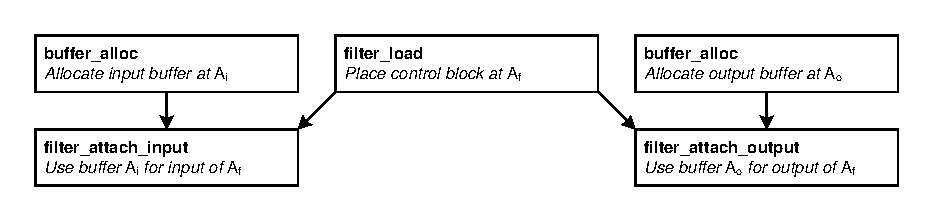
\includegraphics{figs/init}
\end{center}
\caption[Commands to set up a filter.]{Commands to load a filter and allocate and attach input and output buffers. Lines between commands represent dependencies that must be specified to the library when the commands are issued. These commands may be issued in one or multiple groups. See appendix~\ref{app:ui} for detailed information on setting up commands and dependencies.}
\label{fig:lib:init}
\end{figure}

In addition, input data must be transferred into the input buffer before the filter can be run, and output data must eventually be transferred out of the output buffer. With an initially empty input buffer, the commands to transfer in $n$ iterations of input, run the filter for $n$ iterations, and then transfer out $n$ iterations of output (assuming that the input and output buffers were sized appropriately) are shown in figure~\ref{fig:lib:run}.

\begin{figure}[!htb]
\begin{center}
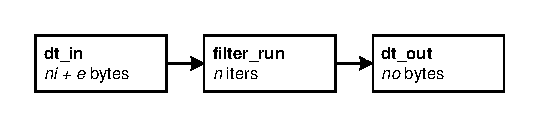
\includegraphics{figs/run}
\end{center}
\caption[Commands to run a filter.]{Commands to run a filter for the first $n$ iterations, including transferring input and output. The corresponding data transfer commands on other SPEs or the PPE are not shown.}
\label{fig:lib:run}
\end{figure}

To run the filter for a larger number of iterations, a sequence of commands is required due to the limited buffer space available in SPE local store. This is illustrated in figure~\ref{fig:lib:ext}.

\begin{figure}[!htb]
\begin{center}
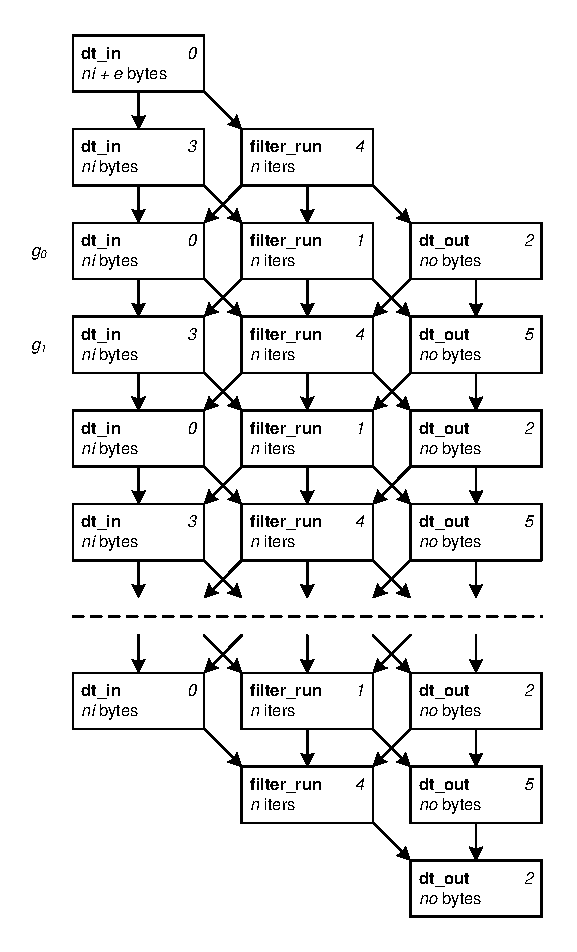
\includegraphics{figs/ext}
\end{center}
\caption[Sequence of commands to run a filter for a large number of iterations.]{Sequence of commands to run a filter for a large number of iterations. Command IDs are indicated in the upper right. Each row is issued as a different group.}
\label{fig:lib:ext}
\end{figure}

Provided that the input buffer is at least $2ni+e$ bytes and the output buffer is at least $2no$ bytes, the dependencies among the commands in the sequence ensure that:
\begin{itemize}
\item When a \textsf{dt\_in} command becomes active, there are at most $ni+e$ bytes of data in the input buffer, and thus enough space to transfer in an additional $ni$ bytes.
\item When a \textsf{dt\_out} command becomes active, there are at least $no$ bytes of data in the output buffer, and thus enough data to transfer out.
\item When a \textsf{filter\_run} command becomes active, there are at least $ni+e$ bytes of data in the input buffer and at most $no$ bytes of data in the output buffer. This is enough input data and output space to run the filter for $n$ iterations.
\end{itemize}

This sequence of commands effectively ``pipelines'' the basic operation from figure~\ref{fig:lib:run}. Double-buffering is accomplished when the data transfer commands in a group complete before the \textsf{filter\_run} does. In this case, the following \textsf{filter\_run} has no outstanding dependencies once the current \textsf{filter\_run} completes, and can become active immediately.

The user can keep the SPE continually supplied with work by initially issuing the first two groups, thereafter issuing the next group whenever a group completes. In this case, the SPE almost always has two groups of commands issued, with one group active and the other queued. In addition, with the exception of the first two and last two groups, the command parameters, IDs and dependencies in every other group are identical. This allows the user to initially set up two groups ($g_0$ and $g_1$ in figure~\ref{fig:lib:ext}) and repeatedly issue them for a majority of the execution. If executions are relatively long, the overhead of the first and last group, where no filter is being run, will be amortized effectively. Alternatively, the user can load another filter and run it during those gaps.

In practice, situations such as the above, where a static-rate filter is run for a large number of iterations and large amounts of input and output data are transferred, are very common. To avoid requiring the user to manually issue groups and deal with command completion callbacks in every such case, the library also provides extended operations that encapsulate this pattern. In an extended operation, the user provides the library with filter rates, the addresses of opposing buffers on other processors for data transfers, and the number of groups to run for; the library issues and responds to all commands internally and notifies the user when the entire operation is complete. Where one or both opposing buffers are located in memory, the library also handles the PPE side of data transfers internally. Extended operations greatly simplify setting up pipelines of any length where all filters in the pipeline have static rates.

\section{Library Implementation}

The library is implemented as three separate components: \emph{i}) runtime code for SPEs, \emph{ii}) basic runtime code for the PPE, and \emph{iii}) runtime code for the PPE that handles extended operations.

\subsection{PPE Implementation}

For each SPE, the library maintains a fixed table of command groups in memory. Each entry in the table represents a group and stores command data for commands in the group. When the user issues a group to an SPE, the library sends a mailbox message to the SPE to notify it of the entry in the table that contains the group and the LS address to copy command data to; the use of a fixed table is directly necessary to be able to pack all required fields into a single 32-bit mailbox message. After receiving the mailbox message, library code on the SPE initiates DMA to copy command data into local store.

When commands are completed by an SPE, library code on the SPE sends a bitmap of the command ID(s) to the PPE via the outbound mailbox. If the mailbox is full (the PPE has not had time to respond to the previous message), the bitmap is queued and sent when the mailbox is empty. The size of a mailbox message (32 bits) currently imposes a strict limit on the range of valid command IDs.

Library code on the PPE continually polls the outbound mailboxes of all SPEs in round-robin order for command completion messages. When a message is received, it is processed by the library, which eventually runs the user-registered callback. Interrupts were not used as each interrupt requires approximately 7 $\mu$s of kernel time to process. Although this may be negligible when only a single SPE is involved, it can become significant when multiple SPEs are all generating interrupts. In general, it is the author's opinion that the Cell architecture's focus on directly using SPEs to run small pieces of application code is not suited for the additional system overhead of interrupts.

One major drawback of the continuous polling approach is that it severely constrains any other work that the PPE is able to perform unless the user is willing to call the library function that performs polling at regular intervals. This is not a problem when the PPE is used solely as a control processor; most control computations are in response to command completion messages from SPEs and can be done in the callback.

The sequence of events that occurs on the PPE and an SPE between the time the user issues a group of commands and the user being notified of the completion of a command in the group via callback is illustrated in figure~\ref{fig:lib:control}. In actuality, because \emph{i}) each SPE is issued multiple commands and \emph{ii}) the PPE is controlling multiple SPEs, there will typically be many different copies of this sequence interleaved within each other, for both the same and different SPEs.

\begin{figure}[!htb]
\setstretch{1.5}
\begin{center}
\begin{tabular}{rp{2.5in}p{2.5in}}
& \emph{PPE} & \emph{SPE} \\
\cline{2-3}
& Continually polls for command completion messages from SPEs. & Continually polls for mailbox messages while running active commands. \\
\cline{2-3}
\textsf{(1)} & \emph{User creates new group and adds commands.} Command data is written to entry in groups table. & \\
& \emph{User issues group.} Sends mailbox message to SPE. & \\
& & Receives and unpacks mailbox message. Copies command data (using DMA) from table entry to local store at specified LS address. \\
& & After copying command data, adds new commands to dependency graph. \\
& & \multicolumn{1}{c}{$\cdots$} \\
& & When command(s) complete, writes bitmap of completed ID(s) to PPE. \\
& Receives command completion message and calls user-defined callback. & \\
& \emph{Inside callback, user sets up and issues new groups if desired.} Repeats from \textsf{(1)}. &
\end{tabular}
\end{center}
\caption[SPE control protocol.]{SPE control protocol. \emph{Italicized} text represents actions performed by user code. All other actions are performed by library code.}
\label{fig:lib:control}
\end{figure}

\subsection{SPE Implementation}

To execute multiple active commands concurrently on an SPE, the library implements what is effectively a simple co-operatively multitasked ``operating system''. Each type of command has an associated handler function that processes it, and all active commands on an SPE act as separate ``threads'' executing at separate points in their handler functions, using command data to store temporary state in lieu of a separate stack.

The library maintains a run list that contains all active commands in a circular linked list. At the top level, the library cycles through each command in the run list and calls its handler. Each handler performs a small amount of work, typically only part of the work the command specifies, and then returns to the run list to allow other commands to execute. For example, the handler for the \textsf{filter\_run} command runs the filter's work function for one iteration\footnote{To reduce library overhead for filters that have small work functions, the command actually accepts an additional parameter that specifies the number of iterations to run the work function in each cycle through the run list. Alternatively, the compiler can coarsen the work function directly.} and then returns, relinquishing control of the SPE to other commands; in total, the filter's work function is run once for every cycle through the run list. More complex command handlers, such as those for data transfer commands, implement a simple state machine, storing state variables in temporary space in command data. Commands that are queued (have dependencies that have not yet completed) are not placed on the run list and incur no overhead for commands that are running; this allows the user to queue commands according to convenience, with no penalty.

Commands that perform DMA, such as data transfer commands, can wait for DMA operations to complete after starting them. While waiting, the command is removed from the run list, incurring no overhead for commands that are still running. The SPE continues to run other active commands while the DMA is in progress, providing communication--computation concurrency. Once the DMA operation completes, the command is re-added to the run list and the state machine in the command handler will continue where it left off.

DMA completions and inbound mailbox messages are checked via polling instead of interrupts. The library framework allows this internal functionality to be implemented simply as other commands:
\begin{itemize}
\item A command that polls for DMA completions and wakes other commands. This command also sends queued command completion messages to the PPE.
\item A command that polls the inbound mailbox for new command groups from the PPE. This command must perform DMA to copy command data for the group into local store, and does so using the standard mechanism.
\end{itemize}

The library framework causes polling to be done once every cycle through the run list.

From an implementation perspective, the framework does not seem to add significant complexity. In particular, the handlers for data transfer commands have a number of states and consist of a large outer \textsf{switch} statement. However, data transfers, which involve waits, would be fairly complex in any case, and the only obfuscation forced by the framework is that the otherwise linear structure of the handler function is broken up by \textsf{switch} cases. The framework has the advantage of treating all commands uniformly -- any command handler can perform a data transfer -- and thus it allows the library to be easily extended with new commands.

From an efficiency perspective, the run list involves multiple branches that cannot be predicted and does add some overhead to an SPE's main task of running filter work functions. However, this is generally a small fraction of the time spent in even slightly computation-intensive work functions. The run list framework is also not fair in scheduling multiple \textsf{filter\_run} commands: instead of sharing the SPE equally, they are given time proportional to the time spent in a single iteration of their work functions. However, even a single active \textsf{filter\_run} command makes full use of an SPE, and there is commonly only a single running filter (in addition to data transfer commands).

The library completely avoids interrupts, and consequently relies on co-operative multitasking. This was done for a number of reasons. Foremost, the granularity of a filter work function, which typically performs a small amount of work, provides a natural unit of time for switching between commands. SPEs have no timer interrupt; regardless, no timer interrupt could provide the granularity required: a work function of a typical filter might take tens of microseconds to run. In addition, the large number of registers on SPEs makes register saving and restoring time-consuming if interrupts were to be used for DMA completions and inbound mailbox messages. The current framework also avoids any possibility of race conditions when implementing data transfer commands that access buffers: when a data transfer command handler is executing, all filters are between work function iterations and it is the only code accessing the buffer's head and tail pointers.

Since polling is done only at one specific point in the run list, additional latency is introduced into commands that perform DMA. However, this has no effect as long as the user can overlap data transfer commands with computation.
 
Library code occupies approximately the first 16 KB of local store. The remainder is available for use by filter code, filter state, buffers, and the stack.

\subsection{Data Transfer Implementation}

Data transfer between two buffers on different processors involves additional synchronization between the processors. In particular, the source processor communicates to the destination SPE (SPE to memory data transfer will be discussed later later) \emph{i}) that data is available in the source buffer and \emph{ii}) the value of the source buffer's head pointer, so the destination buffer knows where to copy data from. The interaction between a pair of corresponding data transfer commands is given in figure~\ref{fig:lib:dt}:

\begin{figure}[!htb]
\setstretch{1.5}
\begin{center}
\begin{tabular}{p{2.5in}p{2.5in}}
\emph{Source} & \emph{Destination} \\
\hline
Writes head pointer (using DMA) to destination buffer's control block. & Polls for head pointer from source processor. \\
Polls for acknowledgement from destination SPE. & \\
& After receiving head pointer, starts DMA for actual data. \\
& After copying all data, writes acknowledgement to source buffer's control block. \\
After receiving acknowledgement, completes. & After write completes, completes.
\end{tabular}
\end{center}
\caption{SPE--SPE data transfer protocol.}
\label{fig:lib:dt}
\end{figure}

The actual copying of data is done in a ``pull'' manner by the destination SPE. The entire transfer may require more than one DMA operation when the total transfer size is larger than Cell's maximum 16 KB DMA size, or when either buffer wraps around. After starting a single DMA operation, the destination SPE waits for it to complete before starting the next (during this time, the command is removed from the run list and incurs no overhead).

Polling on both processors is done by checking the control block in the command handler and, if not successful, immediately returning to the run list. The next poll occurs when the command handler is run again the next time through the run list.

Transfers where the source buffer is located in memory (and thus handled by the PPE) differ slightly from the protocol presented above. The PPE can use the completion of the data transfer command on the destination SPE as the acknowledgement.

Transfers where the destination buffer is located in memory require separate handling. Although the PPE can start DMA operations from SPE local store, PPE-initiated DMA is less efficient and having PPE code handle transfers places an additional load on the PPE, which must service all SPEs. Instead, transfers to memory are performed in a ``push'' manner that is approximately the reverse of the protocol described above. The PPE uses the completion of the data transfer command on the source SPE as the acknowledgement; in this manner, polling other than for command completion messages is completely avoided on the PPE and multiple transfers to/from memory place no extra overhead on the PPE.

A single active data transfer command on an SPE does not make full use of the MFC, since it starts a single DMA operation and waits for it to complete before starting another. However, this is offset by two considerations: \emph{i}) there should typically be at least two active data transfer commands, one for the input and one for the output buffers and \emph{ii}) when double-buffering is done via the dependency graph, the slight increase in data transfer latency should have no effect.

For double-buffering to be successful, a \textsf{filter\_run} command that is active concurrently with data transfer commands must return to the run list enough times for the data transfer commands to be able to run completely. As a consequence, \textsf{filter\_run} commands should specify at least three or four iterations. In practice, most filter work functions produce and consume relatively small amounts of data per iteration, and this can be easily met even with relatively small buffer sizes.

\subsubsection{Unaligned Data Transfers}

Data transfers that do not begin on a quadword boundary\footnote{Where the head pointer of the source buffer and the tail pointer of the destination buffer are not aligned on a quadword.} require special handling, since the Cell architecture requires DMA operations of quadword size or larger to be quadword-aligned. It is not safe to DMA the entire quadword that contains the source buffer's head pointer directly into the destination buffer, since this overwrites data before the end of the destination buffer with data from before the front of the source buffer, which may be invalid (figure~\ref{fig:lib:dtua}a). Treating the unaligned portion of this quadword as a series of 1-, 2-, 4-, and 8-byte DMA operations (figure~\ref{fig:lib:dtua}b) produces a large amount of DMA overhead and is a poor use of Cell's communication network.

\begin{figure}[!htb]
\begin{center}
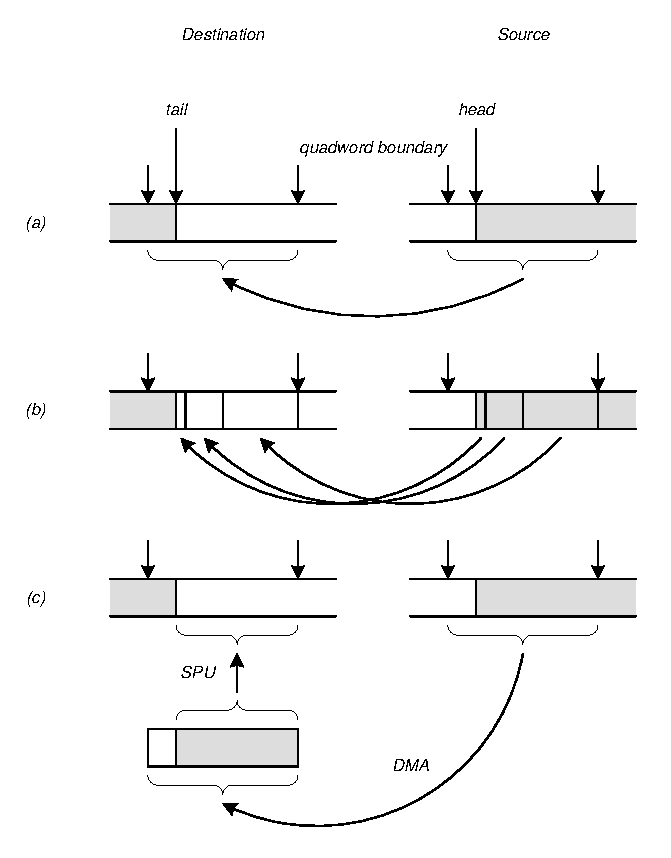
\includegraphics{figs/dt}
\end{center}
\caption[Different ways of handling unaligned data transfers.]{Different ways of handling unaligned data transfers. (a) is incorrect, since it overwrites data in the destination buffer with invalid data from the source buffer. (b) is correct but involves many DMA operations, and is less efficient. (c) is the actual method implemented.}
\label{fig:lib:dtua}
\end{figure}

Instead, the destination SPE DMAs the quadword from the source buffer into the destination buffer's control block, instead of directly into the buffer. When the DMA completes, the destination SPE writes only the valid portion of quadword into the destination buffer.\footnote{This is actually a read-modify-write operation, but it is done by the SPU, not the MFC.} This is illustrated in figure~\ref{fig:lib:dtua}c. The library uses intrinsics to avoid an expensive \textsf{for} loop. For transfers to a destination buffer located in memory, the source SPE DMAs the quadword to the destination buffer's control block and the PPE writes the valid portion of the quadword into the destination buffer using VMX intrinsics after the source command completes.
